% 第 12 题（5）解析：z-U 图像（pgfplots，数据描点 + 线性拟合）
% 数据来自题表 10 组测量值
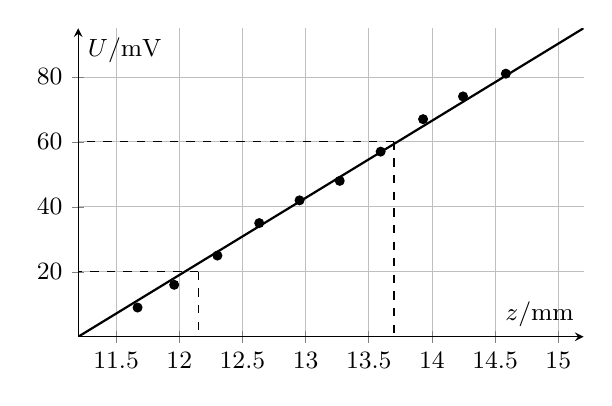
\begin{tikzpicture}
  \begin{axis}[
      width=8cm, height=5.5cm,
      axis lines=middle,
      xlabel={$z$/mm}, ylabel={$U$/mV},
      xmin=11.2, xmax=15.2, ymin=0, ymax=95,
      xtick={11.5,12,12.5,13,13.5,14,14.5,15},
      ytick={0,20,40,60,80},
      grid=both, grid style={line width=0.3pt, draw=gray!50},
      font=\small]
    \addplot[only marks, mark=*, mark size=1.6pt] coordinates {
      (11.670,9) (11.960,16) (12.302,25) (12.633,35) (12.952,42)
      (13.270,48) (13.594,57) (13.930,67) (14.246,74) (14.585,81)};
    \addplot[thick] coordinates {(11.2,0) (15.2,95)};
    \draw[dashed] (12.15,20) -- (12.15,0) node[below] {\small $12.15$};
    \draw[dashed] (12.15,20) -- (11.2,20) node[left] {\small $20$};
    \draw[dashed] (13.70,60) -- (13.70,0) node[below] {\small $13.70$};
    \draw[dashed] (13.70,60) -- (11.2,60) node[left] {\small $60$};
  \end{axis}
\end{tikzpicture}
